\documentclass{article}

% use Times
\usepackage{times}
% For figures
\usepackage{graphicx} % more modern
%\usepackage{epsfig} % less modern
\usepackage{subfigure} 

% For citations
\usepackage{natbib}

% For algorithms
\usepackage{algorithm}
\usepackage{algorithmic}

% As of 2011, we use the hyperref package to produce hyperlinks in the
% resulting PDF.  If this breaks your system, please commend out the
% following usepackage line and replace \usepackage{icml2015} with
% \usepackage[nohyperref]{icml2015} above.
\usepackage{hyperref}

% Packages hyperref and algorithmic misbehave sometimes.  We can fix
% this with the following command.
\newcommand{\theHalgorithm}{\arabic{algorithm}}

% Employ the following version of the ``usepackage'' statement for
% submitting the draft version of the paper for review.  This will set
% the note in the first column to ``Under review.  Do not distribute.''
\usepackage{icml2015stylefiles/icml2015} 

% Employ this version of the ``usepackage'' statement after the paper has
% been accepted, when creating the final version.  This will set the
% note in the first column to ``Proceedings of the...''
%\usepackage[accepted]{icml2015}

\usepackage{tikz}
\usepackage{dsfont}
\usepackage{amsmath}
\usepackage{amssymb}
\usepackage{amsthm}
\usepackage{cleveref}

\graphicspath{ {figures/} }
\usetikzlibrary{arrows,positioning} 
\tikzset{
    %Define standard arrow tip
    >=stealth',
    %Define style for boxes
    observed/.style={
           circle,
           rounded corners,
           draw=black, thick,
           minimum width=2.5em,
           minimum height=2.5em,
           font=\footnotesize,
           text centered,
           fill=blue!20!white},
     latent/.style={
           circle,
           rounded corners,
           draw=black, thick, dashed,
           minimum width=.5em,
           minimum height=.5em,
           font=\footnotesize,
           text centered,
           fill=black!10!white
           },
     empty/.style={
           circle,
           rounded corners,
           minimum width=.5em,
           minimum height=.5em,
           font=\footnotesize,
           text centered,
           },
    % Define arrow style
    pil/.style={
           o->,
           thick,
           shorten <=2pt,
           shorten >=2pt,},
    sh/.style={ shade, shading=axis, left color=red, right color=green,
    shading angle=45 }  
}

\newcommand{\defined}{\vcentcolon =}
\newcommand{\rdefined}{=\vcentcolon}
\newcommand{\E}[1]{\mathbb E\left[#1\right]}
\newcommand{\Var}{\operatorname{Var}}
\newcommand{\calF}{\mathcal F}
\newcommand{\sr}[1]{\stackrel{#1}}
\newcommand{\set}[1]{\left\{#1\right\}}
\newcommand{\ind}[1]{\mathds{1}\!\!\set{#1}}
\newcommand{\argmax}{\operatornamewithlimits{arg\,max}}
\newcommand{\argmin}{\operatornamewithlimits{arg\,min}}
\newcommand{\floor}[1]{\left \lfloor {#1} \right\rfloor}
\newcommand{\ceil}[1]{\left \lceil {#1} \right\rceil}
\newcommand{\eqn}[1]{\begin{align}#1\end{align}}
\newcommand{\eq}[1]{\begin{align*}#1\end{align*}}
\newcommand{\Ber}{\operatorname{Bernoulli}}
\renewcommand{\P}[1]{\operatorname{P}\left\{#1\right\}}
\newcommand{\bigo}[1]{\mathcal{O}\left( #1 \right)}
\newcommand{\bigotilde}[1]{\tilde{\mathcal{O}}\left( #1 \right)}
\newcommand{\bigtheta}[1]{\Theta\left( #1 \right)}
\newcommand{\bigthetatilde}[1]{\tilde{\Theta}\left( #1 \right)}
\newcommand{\bigomega}[1]{\Omega\left( #1 \right)}

\theoremstyle{plain}
\newtheorem{theorem}{Theorem}
\newtheorem{proposition}[theorem]{Proposition}
\newtheorem{lemma}[theorem]{Lemma}
\newtheorem{corollary}[theorem]{Corollary}
\theoremstyle{definition}
\newtheorem{definition}[theorem]{Definition}
\newtheorem{assumption}[theorem]{Assumption}
\newtheorem{remark}[theorem]{Remark}
\newtheorem{example}[theorem]{Example}

% The \icmltitle you define below is probably too long as a header.
% Therefore, a short form for the running title is supplied here:
\icmltitlerunning{Causal Bandits}

\begin{document} 

\twocolumn[
\icmltitle{Casual Bandits}

% It is OKAY to include author information, even for blind
% submissions: the style file will automatically remove it for you
% unless you've provided the [accepted] option to the icml2015
% package.
\icmlauthor{Your Name}{email@yourdomain.edu}
\icmladdress{Your Fantastic Institute,
            314159 Pi St., Palo Alto, CA 94306 USA}
\icmlauthor{Your CoAuthor's Name}{email@coauthordomain.edu}
\icmladdress{Their Fantastic Institute,
            27182 Exp St., Toronto, ON M6H 2T1 CANADA}

% You may provide any keywords that you 
% find helpful for describing your paper; these are used to populate 
% the "keywords" metadata in the PDF but will not be shown in the document
\icmlkeywords{causal,bandit}

\vskip 0.3in
]

\begin{abstract} 

\end{abstract} 

\section{Introduction}
Problems requiring choosing an action under uncertainty are rife in all areas of human endeavour. For many problems, actions may be chosen sequentially, allowing the agent to learn from the outcome of early choices to improve later ones. 

A widely used framework for sequential decision making is the multi-armed bandit. In the classic multi-armed bandit setting there is a finite set of available actions, each associated with a distribution over rewards which is unknown but stationary. At each timestep the agent selects an action and receives a reward sampled i.i.d from the corresponding reward distribution. The performance of bandit algorithms is described by the regret: the difference in the expected reward obtained by the algorithm and the reward that could be obtained if the optimal action was selected at every timestep. 

An an alternate approach to selecting actions is causal inference. Frameworks for causal inference provide a mechanism to specify assumptions that allow observational distributions over variables to be mapped to interventional ones. This allows an agent to predict the outcome of an action based on non-experimental data. This approach is common in social science, demography, and economics where explicit experimentation may be difficult. For example, predicting the effect of changes to childcare subsidies on workforce participation or school choice on student grades. 

We take a first step towards unifying these approaches by considering a variant of the stochastic multi-armed bandit problem where we have prior knowledge of the causal structure governing the available actions. 

A natural way to connect the causal framework with the bandit setting is to model the problem as a causal directed acyclic graph. Each possible assignment of variables to values is an action (bandit arm). The reward could be a general function of the action selected and the final state of the graph. However for simplicity, we will consider the reward to be the value of a single specified node minus the cost of the selected action. The number of actions grows exponentially with the number of variables in the graph, making it important to use algorithms that take account of the graph structure to reduce the search space. 

Problems framed in this way take on characteristics of different bandit settings depending on the assumptions we make about what subset of actions can be taken, what variables are observable and whether they are observed before or after an action is selected. If feedback is received only on the reward node then the do-calculus can be applied to eliminate some actions immediately, before any experiments are performed and then a standard bandit algorithm can be run on the remaining actions. 

If we receive feedback on additional nodes the problem can be more interesting. In addition to being able to eliminate some actions prior to sampling any data as in the previous case, taking one action may give us some information on actions that were not selected. 

We consider a bandit problem where the actions and reward are represented by a specific causal graph that demonstrates this interesting structure. We develop an algorithm to leverage the information provided by this structure and demonstrate it substantially outperforms standard bandit algorithms applied to the same problem where the number of actions is large.

There has been substantial recent work into extending bandit algorithms to incorporate additional assumptions and deal with more complex feedback structures. Algorithms with strong guarantees have been developed for linear bandits [], generalized linear bandits, gaussian process bandits [], etc. There is also an active line of research into bandits with feedback defined by a graph. Actions are modelled as nodes in the graph and the agent observes rewards for each action connected to the selected action []. The novelty of our work is that we assume prior knowledge of the causal structure but not the functional form of the relationship between variables.   

Partial monitoring is a very general framework for for decoupling the feedback from the action and reward. It can be used to classify problems into one of four categories, trivial with no regret, easy with $R_T = \bigthetatilde{\sqrt{T}}$ , hard with $R_T = \bigtheta{T^{2/3}}$ and hopeless with $R_T = \bigomega{T}$ \cite{Bartok2014}. Partial monitoring algorithms yield results that are optimal with respect the the horizon $T$ but not other parameters, such as $K$, which is the key focus of incorporating causal structure. 

ALSO NEED TO MENTION ANY OTHER COMBINATIONS OF BANDITS+CAUSAL (eg the Elias NIPS paper and Generalized Thompson Sampling paper)

Key to Elias' paper is: observing the action an agent would take if it were allowed to make its natural choice can provide some information about hidden confounders that influence both the reward and the choice of action. Therefore, incorporating an agents natural choice as context may outperform a standard bandit that does not use that context. (Note: even in the presence of hidden confounders, including the agents natural choice as context only may improve the results. It is easy to come up with a counter example in which it does not).

\section{Problem setup}

Assume we have a known causal model with binary variables $\boldsymbol{X} = \{X_{1}..X_{N}\}$ that independently cause a target variable of interest $Y$, figure \ref{fig:causalStructure}. We can run sequential experiments on the system, where at each timestep $t$ we can either do nothing, $do()$ \footnote{A note on notation: In the bandit community it is implicit that algorithms selecting actions are intervening in the system. So it is sufficient to index actions according to the variable and value. However, in causal graphs, it is essential to differentiate observing (or conditioning) on a variable taking a certain value, from intervening to set that variable. Although in the specific causal graph we consider, observation and intervention are the same, we deliberately introduce the do-notation \cite{Pearl2000} that makes this distinction clear so as to help provide a bridge between the bandit and causal inference communities.} , or select a single variable, $X_i$, on which to intervene, $do(X_{t,i} = J_t)$, and subsequently observe the complete result, $(\boldsymbol{X}_{t},Y_{t})$. 



As an example, consider a farmer wishing to optimize the yield of her crop. She can invest in a green house to control temperature, a watering system to control soil moisture, fertilizers to set soil nutrients, etc. We assume only a single intervention is feasible due to cost and that each of these variables are independent of one-another (this may not always be the case - temperature could be related to rainfall for example). After having selected which variable to control, she plants her crops and observes the values of the remaining input variables and the yield. This repeats across many growing seasons, and the goal is to maximize the total cumulative yield.

\begin{figure}[h]
\centering
\caption{Assumed Causal Structure}
\label{fig:causalStructure}
\begin{tikzpicture}[->,>=stealth',shorten >=1pt,auto,node distance=1cm,
  thick,main node/.style={observed}, hidden/.style={empty}]

 %nodes
\node[main node](1){$X_{1}$};
\node[main node, right=of 1](2){$X_{2}$};
\node[hidden, right=of 2](3){$...$};
\node[main node, right=of 3](4){$X_{N}$};
\node[main node, below right=of 2](5){Y};
 \path[every node/.style={font=\sffamily\small}]
    (1) edge (5)
    	(2) edge (5)
    (4) edge (5);
	
\end{tikzpicture}
\end{figure}



Let $\boldsymbol{q} \in [0,1]^N$ be a fixed vector where $q_i = P(X_i = 1)$. In each time-step $t$ upto a known end point $T$:
 
\begin{enumerate}
\item The learner chooses $I_t \in \set{0...N}$ and $J_t \in \set{0,1}$, corresponding to setting the variable $X_{I_t}=J_t$, also denoted $do(X_{I_t} = J_t)$. Selecting $I_t = 0$ represents not intervening on any variable and simply observing, also denoted $do()$.

\item The remaining variables take their values stochastically according to their natural probabilities $\boldsymbol{q}$

\eq{
X_{i,t} = \begin{cases}
\sim Bernoulli(q_i) &\text{if } i \neq I_t \\
J_t & \text{otherwise}\,.
\end{cases}
}

\item The learner receives reward $Y_t \sim \Ber(r(\boldsymbol{X}_t))$ where $r:\set{0,1}^N \to [0,1]$ is unknown and arbitrary.
\end{enumerate}

The expected reward of taking action $i,j$ is $\mu_{i,j} = \E{r(X)|do(X_i = j)}$. The optimal reward and action are denoted $\mu^*$ and $(i^*,j^*)$ respectively,
where $(i^*,j^*) = \argmax_{i,j} \mu_{i,j}$ and $\mu^* = \mu(i^*,j^*)$. The $n$-step cumulative expected regret is
\eq{
R_n = \E {\sum_{t=1}^n \left(\mu^* - \mu_{I_t,J_t}\right)}.
}

The problem could be treated as a classical multi-armed bandit with $K = 2N+1$ arms, yielding a regret $\bigo{\sqrt{TN}}$. However, this doesn't leverage the side information induced by the causal structure.

\section{Causal Bandits}

Given the assumed causal structure, the probability of $Y_t$ given we intervene to set $X_{i,t} = j$ is the same as if we don't set any variables and observe $X_{i,t} = j$. 

\eqn {
\label{eq:observe}
P(Y_t|do(X_{i,t} = j)) = P(Y_t|do(),X_{i,t} = j)
}

This follows from application of the do-calculus \cite{Pearl2000} to our specific causal graph. It is not the case in general. For example if there was a variable $X'$ that caused both $X_i$ and $Y$ (or $X_i$ and any other variable $X_l$), that would introduce a backdoor path from $X_i \rightarrow Y$ and we would have to condition on $X'$ to derive the interventional distribution of $Y$ from the observational one.

\color{red} Probably should define causal model and back-door rule to properly show this.\color{black}

We can also learn about the reward for intervening on one variable from rounds in which we actually set a different variable.

\eqn {
\label{eq:estimation_transfer}
P(Y_t|do(X_{i,t} = j))= & \nonumber \\
 \sum_{j'}  P(Y_t|do(X_{l,t} & = j'),X_{i,t} = j)P(X_{l_t} = j')
}

We propose a simple explore-exploit based algorithm that leverages  \eqref{eq:observe}. Without loss of generality, we assume $q_i \in [0,\frac{1}{2}]$ and $q_1 \leq q_2 ... \leq q_N$. 

\begin{algorithm}[h]
   \caption{Causal Explore-Exploit}
   \label{alg:known_q}
\begin{algorithmic}
   \STATE {\bfseries Input:} $T,\boldsymbol{q}$
   \STATE Let $m =   min\set{1 \leq i \leq N:q_{i+1} \geq \frac{1}{i}}$
   \STATE Let $h = T^{2/3}m^{1/3}log(TK)^{1/3}$
   \STATE Let $A = \set{(i,j) : i \leq m, j = 1}$ be the set of infrequently observed arms
   \FOR{$t=1$ {\bfseries to} $h/2$}
   \STATE Choose the action $do()$ and observe $\boldsymbol{X}_t$ and $r_t$
   \ENDFOR
   \STATE Compute for all arms $(i,j) \notin A$:
   \eq{
   \hat{\mu}_{i,j} = \frac{2}{h}\frac{\sum_{t=1}^{h/2}\ind{X_{i,t}=j}r_t}{q_i^j(1-q_i)^{1-j}}
   }
   \FOR{$(i,j) \in A$}
    \FOR{$t'=1$ {\bfseries to} $h/2m$}
    \STATE Choose the action $do(X_{i,t'} = j)$ and observe $r_t$
    \ENDFOR
    \STATE Compute $\hat{\mu}_{i,j} = \frac{2m}{h}\sum_{t'=1}^{h/2m}\ind{X_{i,t'} = j}r_{t'}$
   \ENDFOR
   \STATE Compute $(\hat{i}^*,\hat{j}^*) = \argmax_{(i,j)} \hat{\mu}_{i,j}$
   \FOR{$t=h$ {\bfseries to} $T$}
   \STATE Choose the action $do(X_{\hat{i}^*,t} = \hat{j}^*)$
   \ENDFOR
\end{algorithmic}
\end{algorithm}

\begin{theorem}\label{thm:known_q_regret}
Define $m =   min\set{1 \leq i \leq N:q_{i+1} \geq \frac{1}{i}}$
Then \cref{alg:known_q} satisfies
\eq{
R(T) \in \bigo{T^{2/3}m^{1/3}log(KT)^{1/3}}\,.
}
\end{theorem}

The lower bound for the standard bandit problem is $R_t \in \bigomega{\sqrt{TK}}$ \cite{Auer1995}. Comparing these results shows exploiting the extra information provided by the causal structure should outperform standard bandit algorithms when the number of arms is large, $K >> m^{2/3}T^{1/3}$. The parameter $m$ summarizes the vector $\boldsymbol{q}$, and represents the number of actions that occur rarely naturally and thus must be explicitly explored. If $q_1,...,q_N = 0$, the problem is completely unbalanced and $m = N$. If $q_1,...,q_N = \frac{1}{2}$, the problem is completely balanced and $m = 1$.

Algorithm \ref{alg:known_q} tries to learn the rewards for all the arms during an exploration phase $h$ and then picks the arm with the highest empirical mean for all remaining timesteps. During its exploration phase, it learns all the frequently occurring actions by observation and the remaining, infrequently occurring actions, by explicitly playing them. This leads to Chernoff type high probability bounds on the difference between the empirical and true rewards for all arms of the form $P(\hat{\mu}_{i,j} - \mu_{i,j} > D) \leq e^{-hD^2/m}$. By choosing optimal values for $D$ and $h$ we obtain the regret bound given in \cref{thm:known_q_regret}. A full proof is given in the supplementary materials. 

Algorithm \ref{alg:known_q} relies on $\boldsymbol{q}$ and thus $m$ being known. We now consider the case where $\boldsymbol{q}$ is unknown. We begin by considering the simple regret, defined as the expected difference between the mean payoff of the optimal action and that of the action estimated to be optimal in $T$th round. 

\eqn{
R^{simple}(h) = \E{\mu^* - max_{(i,j)}\hat{\mu}_{i,j}(h)}
}

\begin{algorithm}[h]
\caption{Causal Best Arm Identification}\label{alg:simple}
\begin{algorithmic}[1]
\STATE {\bf Input:} $T, N$
\FOR{$t \in 1,\ldots,T/2$}
\STATE Choose the action $do()$ and observe $\boldsymbol{X}_t$ and $r_t$
\ENDFOR
\STATE Compute for all $i \in \set{1,\ldots,N}$ and $j \in \set{0,1}$:
\eq{
\hat \mu_{i,j} = \frac{\sum_{t=1}^{T/2} \ind{X_{i,t} = j} r_t}{\sum_{t=1}^{T/2} \ind{X_{i,t} = j}}\,.
}
\STATE Compute $\hat q_i = \frac{2}{T} \sum_{t=1}^{T/2} X_{i,t}$
\STATE Compute $\hat s_i = \min\set{\hat q_i, 1 - \hat q_i}$
\STATE Compute $\hat{s'} = sorted(\hat{s}) : \hat{s'}_1 \leq \hat{s'_2} \leq ... \leq \hat{s'}_N$
\STATE Compute $\hat m = \min\set{1 \leq i \leq N : \hat s'_{i+1} \geq \frac{1}{i}}$
\STATE $i'(i) = $ the index of $\hat s_i$ in $\hat s'$
\STATE Compute $A$ as the subset of infrequently observed arms $\{(i,j):i'(i) \leq \hat m, j = \ind{\hat q_{i} \leq \frac{1}{2}} \}$ with $|A| = \hat m$

\FOR{$(i,j) \in A$}
\FOR{$t \in 1,\ldots,T/2\hat m$}
\STATE Choose action $do(X_{i,t} = j)$ and observe $r_t$
\ENDFOR
\STATE Recompute $\hat \mu_{i,j} = \frac{2\hat m}{T} \sum_{t=1}^{ T/2\hat m} r_t(X_{i,t}=j)$ 
\ENDFOR
\end{algorithmic}
\end{algorithm}

\begin{theorem}\label{thm:unknown_q_simpleregret}
Define $m =   min\set{1 \leq i \leq N:q_{i+1} \geq \frac{1}{i}}$.
Then \cref{alg:simple} satisfies
\eq{
R^{simple}(T) \in \bigo{\sqrt{\frac{m}{T}log\left(\frac{NT}{m}\right)}}\,.
}
\end{theorem}

The simple regret for a K-armed bandit is lower bounded by $\bigo{\sqrt{K/T}}$ \cite{Bubeck2009}. By utilizing the causal structure the dependence on $K$ is reduced to a dependence on $m$, which may be much smaller. The intuition behind \cref{alg:simple} is that we can use data collected during rounds where we select the $do()$ action to estimate $m$ and determine which arms we must play explicitly. 

For the bandit problem problem we need to collect some data to estimate $m$ before determining if we should use the causal explore-exploit algorithm or a standard bandit algorithm. 


\begin{algorithm}[h]
\caption{Bandit Regret Algorithm}\label{alg:bandit}
\begin{algorithmic}[1]
\STATE {\bf Input:} $T, N$
\STATE $\delta = \frac{1}{T^{1/3}}$ 
\STATE $T_1 = 48Nlog\left(4N/\delta\right)$ 
\STATE Run \cref{alg:simple} to line 11 with input $T_1,N$.
\IF {$\hat{m} > \frac{N^{3/2}}{\sqrt{T}}$}
\STATE Switch to the standard UCB algorithm.
\ELSE
\STATE $h = T^{2/3}\hat{m}^{1/3}log(TK)^{1/3}$ 
\STATE Run \cref{alg:simple} with input $h,N$.
\STATE Compute $(\hat{i}^*,\hat{j}^*) = \argmax_{(i,j)} \hat{\mu}_{i,j}$
\FOR{$t=h$ {\bfseries to} $T$}
\STATE Choose the action $do(X_{\hat{i}^*,t} = \hat{j}^*)$
\ENDFOR
\ENDIF
\end{algorithmic}
\end{algorithm}

\begin{theorem}\label{thm:unknown_q_regret}
Define $m =   min\set{1 \leq i \leq N:q_{i+1} \geq \frac{1}{i}}$
Then \cref{alg:bandit} satisfies
\eq{
R(T) \in \bigo{T^{2/3}m^{1/3}log(KT)^{1/3}}\,.
}
\end{theorem}

\subsection{Lower Bounds}

\section{Experiments}

\begin{figure}
\caption{Final regret versus number of variables $N$ for UCB with $\alpha = 2$, Causal-Explore-Exploit with $m=2$ and with $m=N$ and horizon $T = 10,000$ . Error bars show standard deviation over 100 simulations. The regret for UCB grows linearly with the number of variables, whist for Causal-Explore-Exploit with fixed $m$, the growth is sub-logarthmic.  }
\label{fig:known_q_r_vs_N}
\centering
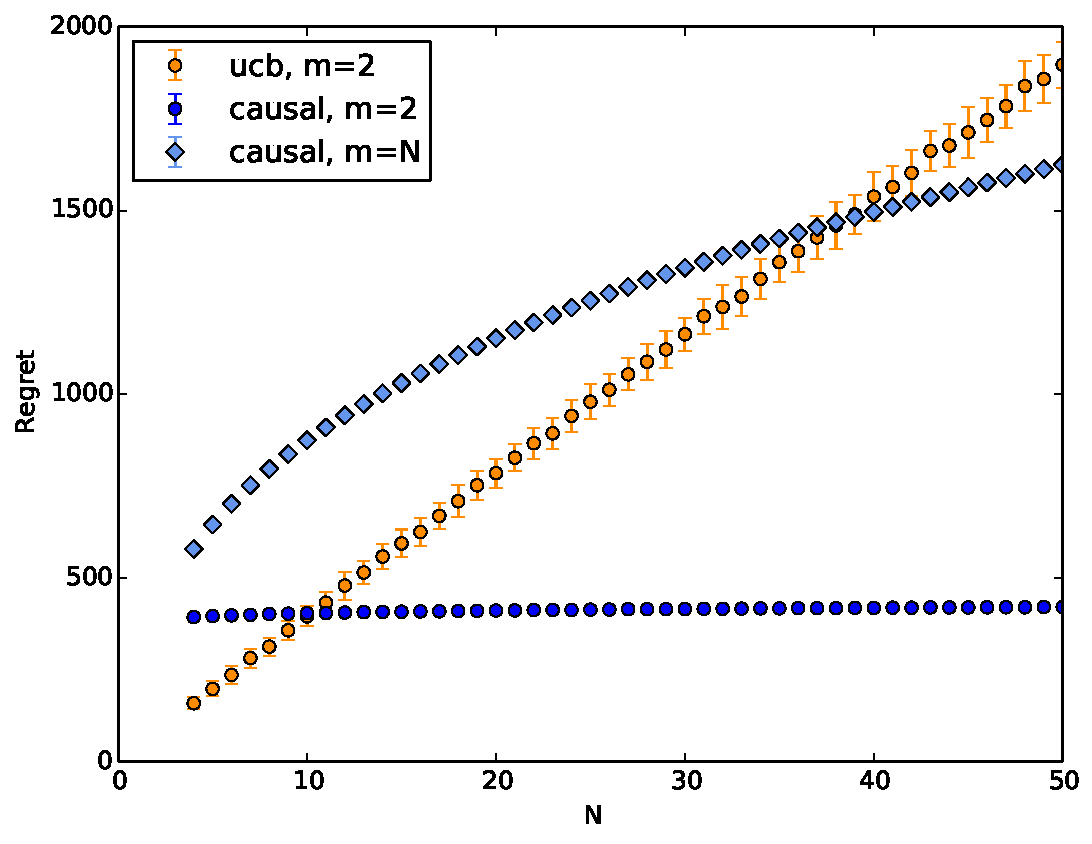
\includegraphics[width=.5\textwidth]{exp_regret_vs_N_T10000_sims100_20151229_113550.pdf}
\end{figure}

\begin{figure}
\caption{Cumulative regret over time for $N = 17$ for UCB with $\alpha=2$, Causal-Explore-Exploit with $m=2$ and Causal-Explore-Exploit with $m=N$. Shaded region shows standard deviation over 100 simulations. The Causal-Explore-Exploit algorithm incurs linear regret during the exploration phase, after which it selects the optimal arm with high probability. For $m=2$, we have $K \sim m^{2/3}T^{1/3}$ and see that we are in the regime in which Causal-Explore-Exploit outperforms UCB.}
\label{fig:known_q_r_vs_t}
\centering
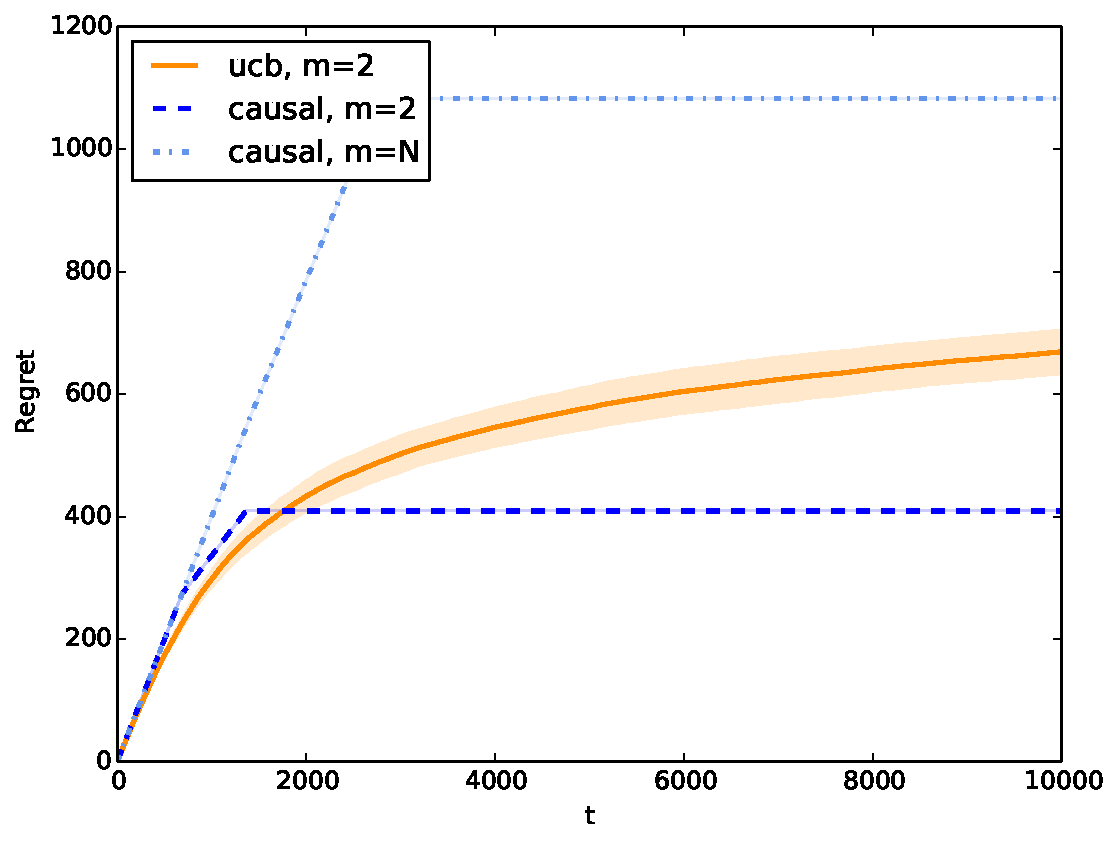
\includegraphics[width=.5\textwidth]{exp_regret_vs_t_T10000_N17_sims100_20151229_120647.pdf}
\end{figure}


\section{Discussion}


In our algorithm, we have only used the side information provided by the $do()$ action about other actions. Since the $do()$ action fully reveals the value of alternate actions we could have incorporated this information via the graph feedback model \cite{Mannor2011}, where at each timestep the feedback graph $G_t$ is selected stochastically, dependent on $\boldsymbol{q}$, and revealed after an action has been chosen. The feedback graph is distinct from the causal graph. A link $A \rightarrow B$ in $G_t$ indicates that selecting the action $A$ reveals the reward for action $B$. For this specific problem, $G_t$ will always be a star graph with the action $do()$ connected to half the remaining actions. The Exp3-IX algorithm \cite{Kocak2014} was developed for the adversarial version of this problem and has regret $\bigo{\sqrt{\bar{\alpha}T}}$, where $\bar{\alpha}$ is the average independence number of $G_t$. In our case $\bar{\alpha} = \frac{N}{2}$ so we again obtain the regret of the standard bandit algorithm. The issue here is that a malicious adversary can select the same graph each time, such that the rewards for half the arms are never revealed by the informative action. This is equivalent to a, nominally, stochastic selection of feedback graph where $\boldsymbol{q} = \boldsymbol{0}$

\cite{Lelarge2012} consider a stochastic version of the graph feedback problem, but with a fixed graph available to the algorithm before it must select an action. In addition, their algorithm is not optimal for all graph structures and fails, in particular, to provide improvements for star like graphs as in our case. \cite{Buccapatnam2014} improve the dependence of the algorithm on the graph structure but still assume the graph is fixed and available to the algorithm before the action is selected. 

More generally, assuming causal structure creates more complex types of side information, such as that shown in equation \ref{eq:estimation_transfer}. In this case, selecting one action does not fully reveal an alternate action but provides some information towards an estimate. The quality of the estimate notably depends not only on the number of times that action was selected. For example, to get a good estimate for $X_1 = 1$ by intervening on $X_2$ requires us to sample both $X_2=0$ and $X_2=1$, in proportions dependent on $q_2$. This more complex side information does not fit within the graph feedback framework.


\section{Future Open Questions}
\begin{itemize}
\item Known but arbitrary structure
\item Learning structure then exploiting
\end{itemize}
\section{Conclusion}


\end{document}